\documentclass[]{book}
\usepackage{lmodern}
\usepackage{amssymb,amsmath}
\usepackage{ifxetex,ifluatex}
\usepackage{fixltx2e} % provides \textsubscript
\ifnum 0\ifxetex 1\fi\ifluatex 1\fi=0 % if pdftex
  \usepackage[T1]{fontenc}
  \usepackage[utf8]{inputenc}
\else % if luatex or xelatex
  \ifxetex
    \usepackage{mathspec}
  \else
    \usepackage{fontspec}
  \fi
  \defaultfontfeatures{Ligatures=TeX,Scale=MatchLowercase}
\fi
% use upquote if available, for straight quotes in verbatim environments
\IfFileExists{upquote.sty}{\usepackage{upquote}}{}
% use microtype if available
\IfFileExists{microtype.sty}{%
\usepackage{microtype}
\UseMicrotypeSet[protrusion]{basicmath} % disable protrusion for tt fonts
}{}
\usepackage[margin=1in]{geometry}
\usepackage{hyperref}
\hypersetup{unicode=true,
            pdftitle={An Introduction to Inertial Sensors Stochastic Calibration},
            pdfauthor={Stéphane Guerrier, Roberto Molinari, Yuming Zhang, Haotian Xu, Gaetan Bakalli, Ahmed Radi and Mucyo Karemera},
            pdfborder={0 0 0},
            breaklinks=true}
\urlstyle{same}  % don't use monospace font for urls
\usepackage{natbib}
\bibliographystyle{apalike}
\usepackage{color}
\usepackage{fancyvrb}
\newcommand{\VerbBar}{|}
\newcommand{\VERB}{\Verb[commandchars=\\\{\}]}
\DefineVerbatimEnvironment{Highlighting}{Verbatim}{commandchars=\\\{\}}
% Add ',fontsize=\small' for more characters per line
\usepackage{framed}
\definecolor{shadecolor}{RGB}{248,248,248}
\newenvironment{Shaded}{\begin{snugshade}}{\end{snugshade}}
\newcommand{\AlertTok}[1]{\textcolor[rgb]{0.94,0.16,0.16}{#1}}
\newcommand{\AnnotationTok}[1]{\textcolor[rgb]{0.56,0.35,0.01}{\textbf{\textit{#1}}}}
\newcommand{\AttributeTok}[1]{\textcolor[rgb]{0.77,0.63,0.00}{#1}}
\newcommand{\BaseNTok}[1]{\textcolor[rgb]{0.00,0.00,0.81}{#1}}
\newcommand{\BuiltInTok}[1]{#1}
\newcommand{\CharTok}[1]{\textcolor[rgb]{0.31,0.60,0.02}{#1}}
\newcommand{\CommentTok}[1]{\textcolor[rgb]{0.56,0.35,0.01}{\textit{#1}}}
\newcommand{\CommentVarTok}[1]{\textcolor[rgb]{0.56,0.35,0.01}{\textbf{\textit{#1}}}}
\newcommand{\ConstantTok}[1]{\textcolor[rgb]{0.00,0.00,0.00}{#1}}
\newcommand{\ControlFlowTok}[1]{\textcolor[rgb]{0.13,0.29,0.53}{\textbf{#1}}}
\newcommand{\DataTypeTok}[1]{\textcolor[rgb]{0.13,0.29,0.53}{#1}}
\newcommand{\DecValTok}[1]{\textcolor[rgb]{0.00,0.00,0.81}{#1}}
\newcommand{\DocumentationTok}[1]{\textcolor[rgb]{0.56,0.35,0.01}{\textbf{\textit{#1}}}}
\newcommand{\ErrorTok}[1]{\textcolor[rgb]{0.64,0.00,0.00}{\textbf{#1}}}
\newcommand{\ExtensionTok}[1]{#1}
\newcommand{\FloatTok}[1]{\textcolor[rgb]{0.00,0.00,0.81}{#1}}
\newcommand{\FunctionTok}[1]{\textcolor[rgb]{0.00,0.00,0.00}{#1}}
\newcommand{\ImportTok}[1]{#1}
\newcommand{\InformationTok}[1]{\textcolor[rgb]{0.56,0.35,0.01}{\textbf{\textit{#1}}}}
\newcommand{\KeywordTok}[1]{\textcolor[rgb]{0.13,0.29,0.53}{\textbf{#1}}}
\newcommand{\NormalTok}[1]{#1}
\newcommand{\OperatorTok}[1]{\textcolor[rgb]{0.81,0.36,0.00}{\textbf{#1}}}
\newcommand{\OtherTok}[1]{\textcolor[rgb]{0.56,0.35,0.01}{#1}}
\newcommand{\PreprocessorTok}[1]{\textcolor[rgb]{0.56,0.35,0.01}{\textit{#1}}}
\newcommand{\RegionMarkerTok}[1]{#1}
\newcommand{\SpecialCharTok}[1]{\textcolor[rgb]{0.00,0.00,0.00}{#1}}
\newcommand{\SpecialStringTok}[1]{\textcolor[rgb]{0.31,0.60,0.02}{#1}}
\newcommand{\StringTok}[1]{\textcolor[rgb]{0.31,0.60,0.02}{#1}}
\newcommand{\VariableTok}[1]{\textcolor[rgb]{0.00,0.00,0.00}{#1}}
\newcommand{\VerbatimStringTok}[1]{\textcolor[rgb]{0.31,0.60,0.02}{#1}}
\newcommand{\WarningTok}[1]{\textcolor[rgb]{0.56,0.35,0.01}{\textbf{\textit{#1}}}}
\usepackage{longtable,booktabs}
\usepackage{graphicx,grffile}
\makeatletter
\def\maxwidth{\ifdim\Gin@nat@width>\linewidth\linewidth\else\Gin@nat@width\fi}
\def\maxheight{\ifdim\Gin@nat@height>\textheight\textheight\else\Gin@nat@height\fi}
\makeatother
% Scale images if necessary, so that they will not overflow the page
% margins by default, and it is still possible to overwrite the defaults
% using explicit options in \includegraphics[width, height, ...]{}
\setkeys{Gin}{width=\maxwidth,height=\maxheight,keepaspectratio}
\IfFileExists{parskip.sty}{%
\usepackage{parskip}
}{% else
\setlength{\parindent}{0pt}
\setlength{\parskip}{6pt plus 2pt minus 1pt}
}
\setlength{\emergencystretch}{3em}  % prevent overfull lines
\providecommand{\tightlist}{%
  \setlength{\itemsep}{0pt}\setlength{\parskip}{0pt}}
\setcounter{secnumdepth}{5}
% Redefines (sub)paragraphs to behave more like sections
\ifx\paragraph\undefined\else
\let\oldparagraph\paragraph
\renewcommand{\paragraph}[1]{\oldparagraph{#1}\mbox{}}
\fi
\ifx\subparagraph\undefined\else
\let\oldsubparagraph\subparagraph
\renewcommand{\subparagraph}[1]{\oldsubparagraph{#1}\mbox{}}
\fi

%%% Use protect on footnotes to avoid problems with footnotes in titles
\let\rmarkdownfootnote\footnote%
\def\footnote{\protect\rmarkdownfootnote}

%%% Change title format to be more compact
\usepackage{titling}

% Create subtitle command for use in maketitle
\newcommand{\subtitle}[1]{
  \posttitle{
    \begin{center}\large#1\end{center}
    }
}

\setlength{\droptitle}{-2em}
  \title{An Introduction to Inertial Sensors Stochastic Calibration}
  \pretitle{\vspace{\droptitle}\centering\huge}
  \posttitle{\par}
  \author{Stéphane Guerrier, Roberto Molinari, Yuming Zhang, Haotian Xu, Gaetan
Bakalli, Ahmed Radi and Mucyo Karemera}
  \preauthor{\centering\large\emph}
  \postauthor{\par}
  \predate{\centering\large\emph}
  \postdate{\par}
  \date{2018-06-05}

\usepackage{booktabs}
\usepackage{amsthm}
\makeatletter
\def\thm@space@setup{%
  \thm@preskip=8pt plus 2pt minus 4pt
  \thm@postskip=\thm@preskip
}
\makeatother

\usepackage{amsthm}
\newtheorem{theorem}{Theorem}[chapter]
\newtheorem{lemma}{Lemma}[chapter]
\newtheorem{corollary}{Corollary}[chapter]
\newtheorem{proposition}{Proposition}[chapter]
\newtheorem{conjecture}{Conjecture}[chapter]
\theoremstyle{definition}
\newtheorem{definition}{Definition}[chapter]
\theoremstyle{definition}
\newtheorem{example}{Example}[chapter]
\theoremstyle{definition}
\newtheorem{exercise}{Remark}[chapter]
\theoremstyle{remark}
\newtheorem*{remark}{Remark}
\newtheorem*{solution}{Solution}
\let\BeginKnitrBlock\begin \let\EndKnitrBlock\end
\begin{document}
\maketitle

{
\setcounter{tocdepth}{1}
\tableofcontents
}
\hypertarget{introduction}{%
\chapter{Introduction}\label{introduction}}

TO DO (Introduction to the text)

\hypertarget{timeseries}{%
\chapter{Introduction to Time Series Analysis}\label{timeseries}}

In this chapter, we will provide an introduction to time series
analysis. This chapter is organized with the following outline:

\begin{itemize}
\tightlist
\item
  Definition and descriptive analysis of time series;
\item
  Latent time series processes and composite stochastic process;
\item
  Dependence within time series;
\item
  Concept of stationarity;
\item
  Concept of linear processes;
\item
  Fundamental representations of time series.
\end{itemize}

\hypertarget{time-series}{%
\section{Time Series}\label{time-series}}

\BeginKnitrBlock{definition}[Time Series]
\protect\hypertarget{def:ts}{}{\label{def:ts} \iffalse (Time Series) \fi{}
}A time series is a stochastic process (i.e.~a sequence of random
variables (r.v.)), defined on a common probability space denoted as
\((X_t)_{t = 1,...,T}\) (i.e. \{\(X_1\), \(X_2\), \ldots{}., \(X_T\)\}).
Note that the time \(t\) is not continuous and belongs to discrete index
sets. Therefore, we implicitly assume that

\begin{itemize}
\tightlist
\item
  \(t\) is not random, i.e.~the time at which each observation is
  measured is known, and
\item
  the time between two consecutive observations is constant.

  \EndKnitrBlock{definition}
\end{itemize}

When recording values of a time series over an extended period of time,
it is usually difficult to discern any trend or pattern of the time
series by simply looking at the values. However, when these data points
are displayed on a plot with time on x-axis and \(X_t\) on y-axis, some
features of the time series jump out. So it is often useful to
understand a time series process by performing a \textbf{descriptive
analysis}, especially when we have data of small or moderate size.

When we perform descriptive analysis, we usually check the following in
the time series data/graph:

\begin{itemize}
\tightlist
\item
  Trends

  \begin{itemize}
  \tightlist
  \item
    Seasonal (e.g.~business cycles)
  \item
    Non-seasonal (e.g.~impact of economic indicators on stock returns)
  \item
    Local fluctuation (e.g.~vibrations observed before, during and after
    an earthquake)
  \end{itemize}
\item
  Changes in the statistical properties

  \begin{itemize}
  \tightlist
  \item
    Mean (e.g.~economic crisis)
  \item
    Variance (e.g.~earnings)
  \item
    States (e.g.~bear/bull in finance)
  \end{itemize}
\item
  Model deviations (e.g.~outliers)
\end{itemize}

\BeginKnitrBlock{example}[Johnson and Johnson Quarterly Earnings]
\protect\hypertarget{exm:exampleJJ}{}{\label{exm:exampleJJ}
\iffalse (Johnson and Johnson Quarterly Earnings) \fi{} }A traditional
example of a time series is the quarterly earnings of the company
Johnson and Johnson. In the graph below, we present these earnings
between 1960 and 1980.
\EndKnitrBlock{example}

\begin{Shaded}
\begin{Highlighting}[]
\CommentTok{# Load simts package}
\KeywordTok{library}\NormalTok{(simts)}
\end{Highlighting}
\end{Shaded}

\begin{verbatim}
## 
## Attaching package: 'simts'
\end{verbatim}

\begin{verbatim}
## The following object is masked _by_ '.GlobalEnv':
## 
##     hydro
\end{verbatim}

\begin{Shaded}
\begin{Highlighting}[]
\CommentTok{# Load data}
\KeywordTok{data}\NormalTok{(jj, }\DataTypeTok{package =} \StringTok{"astsa"}\NormalTok{)}
\CommentTok{# Construct gts object}
\NormalTok{jj =}\StringTok{ }\KeywordTok{gts}\NormalTok{(jj, }\DataTypeTok{start =} \DecValTok{1960}\NormalTok{, }\DataTypeTok{freq =} \DecValTok{4}\NormalTok{)}
\CommentTok{# Plot time series}
\KeywordTok{plot}\NormalTok{(jj, }\DataTypeTok{main =} \StringTok{"Johnson and Johnson Quarterly Earnings"}\NormalTok{,}
     \DataTypeTok{ylab =} \StringTok{"Quarterly Earnings per Share ($)"}\NormalTok{) }
\end{Highlighting}
\end{Shaded}

\begin{figure}

{\centering 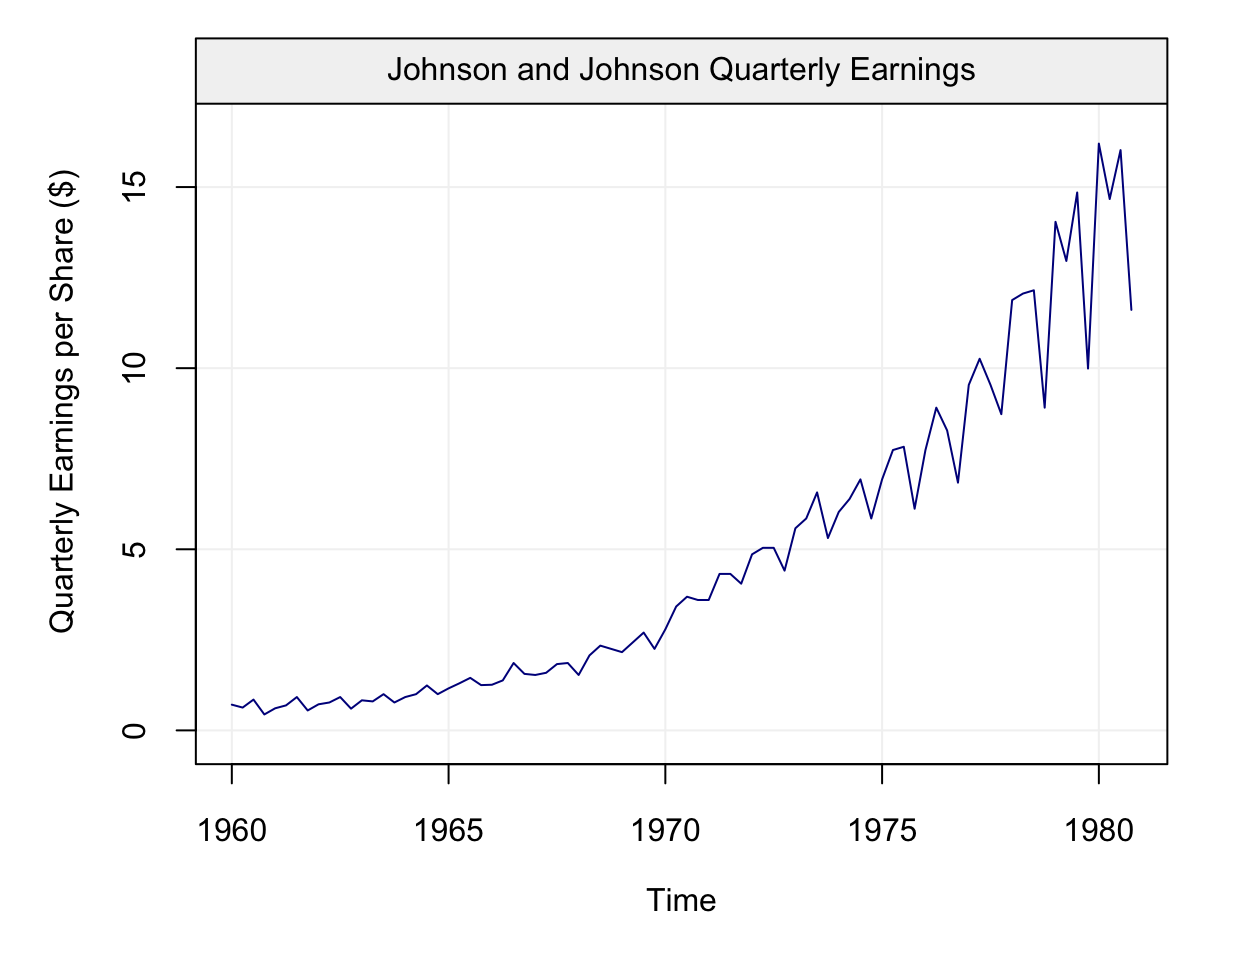
\includegraphics{scis_files/figure-latex/unnamed-chunk-1-1} 

}

\caption{Johnson and Johnson Quarterly Earnings}\label{fig:unnamed-chunk-1}
\end{figure}

As we can see from the graph, the data contains a non-linear increasing
trend as well as a yearly seasonal component. In addition, we can notice
that the variability of the data seems to increase with time. By
plotting the time series graph for this data, we can discern some
important features of the data, which is helpful for us to conduct
further analysis such as selecting suitable models for this data.

\BeginKnitrBlock{example}[Monthly Precipitation Data]
\protect\hypertarget{exm:examplePrecipitation}{}{\label{exm:examplePrecipitation}
\iffalse (Monthly Precipitation Data) \fi{} }Now we consider another
data set coming from the domain of hydrology. The data records monthly
precipitation (in mm) over a certain period of time (1907 to 1972) and
is interesting for scientists in order to study water cycles. The data
are presented in the graph below:
\EndKnitrBlock{example}

\begin{Shaded}
\begin{Highlighting}[]
\CommentTok{# Load data}
\KeywordTok{data}\NormalTok{(hydro, }\DataTypeTok{package =} \StringTok{"simts"}\NormalTok{)}
\CommentTok{# Construct gts object}
\NormalTok{hydro =}\StringTok{ }\KeywordTok{gts}\NormalTok{(hydro, }\DataTypeTok{start =} \DecValTok{1907}\NormalTok{, }\DataTypeTok{freq =} \DecValTok{12}\NormalTok{)}
\CommentTok{# Plot time series}
\KeywordTok{plot}\NormalTok{(hydro, }\DataTypeTok{main =} \StringTok{"Monthly Precipitation Data"}\NormalTok{,}
     \DataTypeTok{ylab =} \StringTok{"Mean Monthly Precipitation (mm)"}\NormalTok{)}
\end{Highlighting}
\end{Shaded}

\begin{figure}

{\centering 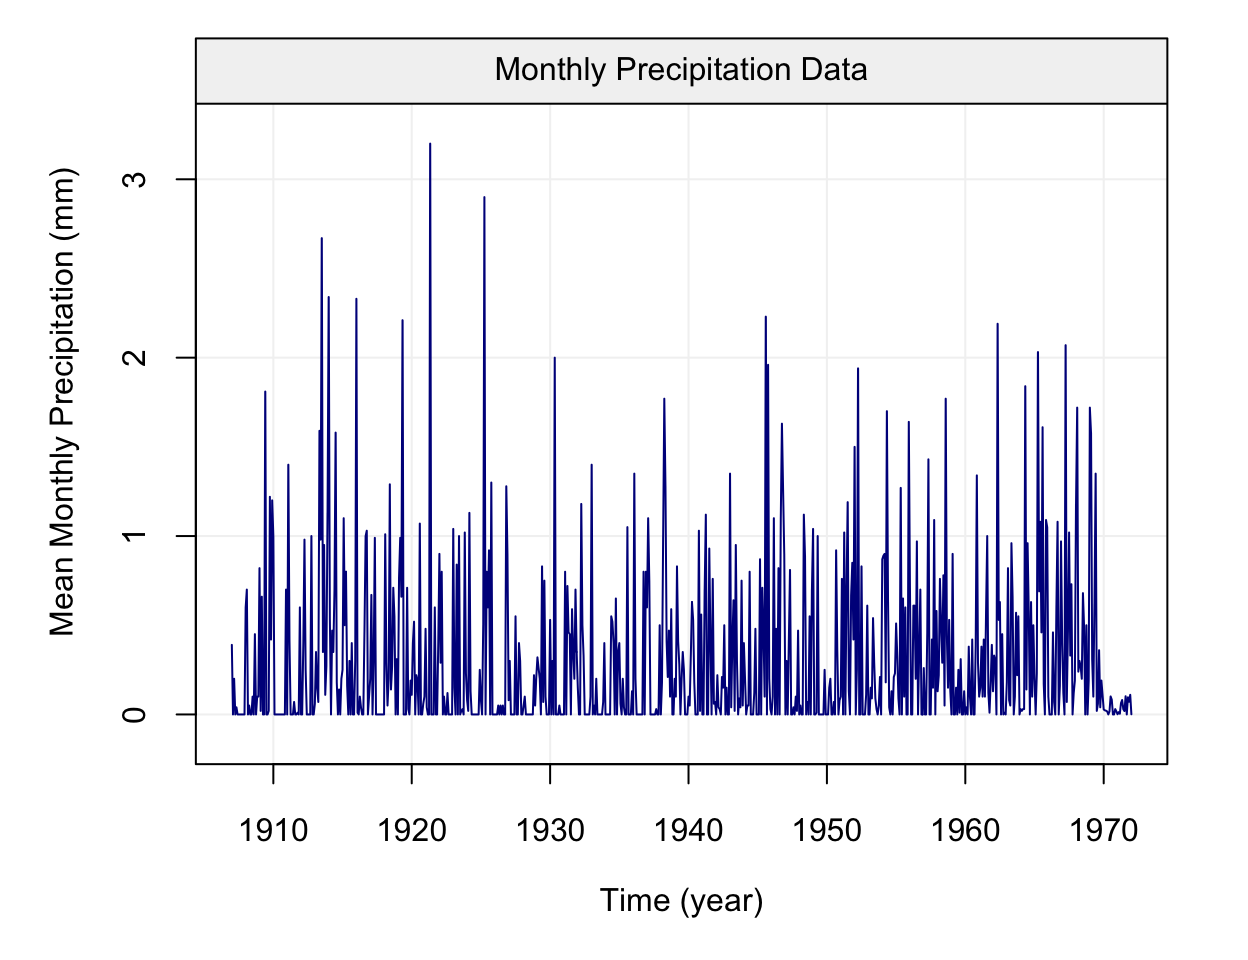
\includegraphics{scis_files/figure-latex/unnamed-chunk-2-1} 

}

\caption{Monthly Precipitation Data}\label{fig:unnamed-chunk-2}
\end{figure}

From the above time series graph, we can observe some extreme
observations (i.e.~outliers) in this data more easily than if we simply
look at all the values of this data.

\BeginKnitrBlock{example}[Inertial Sensor Data]
\protect\hypertarget{exm:exampleInertialSensor}{}{\label{exm:exampleInertialSensor}
\iffalse (Inertial Sensor Data) \fi{} }Now we consider the data coming
from the calibration procedure of an Inertial Measurement Unit (IMU).
The signals coming from an IMU are usually measured at high frequencies
over a long time and are often characterized by linear trends and
numerous underlying stochastic processes. We present the time series
graph of some data from an IMU below.
\EndKnitrBlock{example}

\begin{Shaded}
\begin{Highlighting}[]
\CommentTok{# Load data}
\KeywordTok{data}\NormalTok{(imu6, }\DataTypeTok{package =} \StringTok{"imudata"}\NormalTok{)}
\CommentTok{# Construct gts object}
\NormalTok{imu =}\StringTok{ }\KeywordTok{gts}\NormalTok{(imu6[,}\DecValTok{1}\NormalTok{], }\DataTypeTok{freq =} \DecValTok{100}\OperatorTok{*}\DecValTok{60}\OperatorTok{*}\DecValTok{60}\NormalTok{)}
\CommentTok{# Plot time series}
\KeywordTok{plot}\NormalTok{(imu, }\DataTypeTok{main =} \StringTok{"Inertial Sensor Data"}\NormalTok{,}
     \DataTypeTok{ylab =} \KeywordTok{expression}\NormalTok{(}\KeywordTok{paste}\NormalTok{(}\StringTok{"Error "}\NormalTok{, (rad}\OperatorTok{/}\NormalTok{s}\OperatorTok{^}\DecValTok{2}\NormalTok{))))}
\end{Highlighting}
\end{Shaded}

\begin{figure}

{\centering 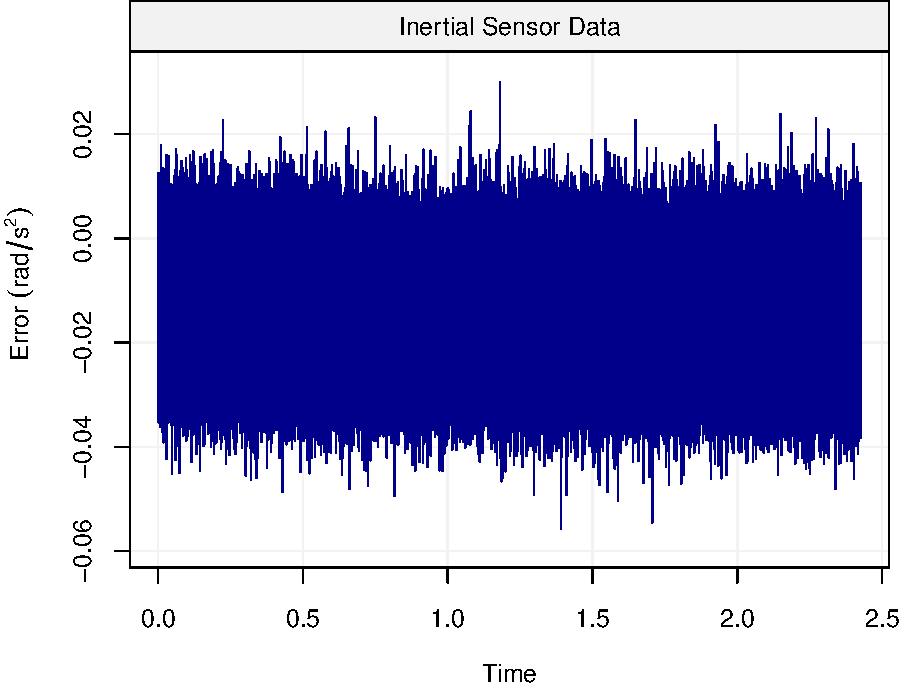
\includegraphics{scis_files/figure-latex/unnamed-chunk-3-1} 

}

\caption{Inertial Sensor Data}\label{fig:unnamed-chunk-3}
\end{figure}

As we can see from the graph, although a linear trend and other
processes are present in this data, it is practically impossible to
discern any feature of the data based on the time series graph. In
general, the descriptive analysis in classical time series analysis is
not appropriate for the analysis of inertial sensors as these data are
usually very large in order to perform parameter estimation.

\hypertarget{latent-time-series-processes-and-composite-stochastic-process}{%
\section{Latent Time Series Processes and Composite Stochastic
Process}\label{latent-time-series-processes-and-composite-stochastic-process}}

We first introduce some latent time series processes that are commonly
used, especially in the calibration procedure of inertial sensors.

\BeginKnitrBlock{definition}[Gaussian White Noise]
\protect\hypertarget{def:WN}{}{\label{def:WN} \iffalse (Gaussian White
Noise) \fi{} }The Gaussian White Noise (WN) process with parameter
\(\sigma^2 \in \mathbb{R}^+\) is defined as \begin{equation*}
        X_t  \overset{iid}{\sim} \mathcal{N}\left(0, \sigma^2 \right)
\end{equation*} where ``iid'' stands for ``independent and identically
distributed''.
\EndKnitrBlock{definition}

\BeginKnitrBlock{definition}[Quantization Noise]
\protect\hypertarget{def:QN}{}{\label{def:QN} \iffalse (Quantization Noise)
\fi{} }The Quantization Noise (QN) process with parameter
\(Q^2 \in \mathbb{R}^+\) is a process with Power Spectral Density (PSD)
of the form \begin{equation*}
        S_{X}(f) = 4 Q^2 \sin^2 \left( \frac{\pi f}{\Delta t} \right) \Delta t, \;\; f < \frac{\Delta t}{2}.
\end{equation*}
\EndKnitrBlock{definition}

\BeginKnitrBlock{definition}[Drift]
\protect\hypertarget{def:DR}{}{\label{def:DR} \iffalse (Drift) \fi{} }The
Drift (DR) process with parameter \(\omega \in \Omega\), where
\(\Omega\) is either \(\mathbb{R}^+\) or \(\mathbb{R}^-\), is defined as
\begin{equation*}
X_t = \omega t.
\end{equation*}
\EndKnitrBlock{definition}

\BeginKnitrBlock{definition}[Random Walk]
\protect\hypertarget{def:RW}{}{\label{def:RW} \iffalse (Random Walk) \fi{}
}The Random Walk (RW) process with parameter
\(\gamma^2 \in \mathbb{R}^+\) is defined as \begin{equation*}
X_t = X_{t-1} + \epsilon_t \;\; \text{where}\;\; \epsilon_t  \overset{iid}{\sim} \mathcal{N}\left(0, \gamma^2 \right)\;\; \text{and}\;\; X_0 = 0.
\end{equation*}
\EndKnitrBlock{definition}

\BeginKnitrBlock{definition}[Auto-Regressive]
\protect\hypertarget{def:AR}{}{\label{def:AR} \iffalse (Auto-Regressive)
\fi{} }The Auto-Regressive process of Order 1 (AR1) with parameter
\(\phi \in (-1, +1)\) and \(\upsilon^2 \in \mathbb{R}^+\) is defined as
\begin{equation*}
X_t = \phi X_{t-1} + Z_t, \;\;\; Z_t \overset{iid}{\sim} \mathcal{N}(0,\upsilon^2).
\end{equation*}
\EndKnitrBlock{definition}

\BeginKnitrBlock{definition}[Gauss Markov]
\protect\hypertarget{def:GM}{}{\label{def:GM} \iffalse (Gauss Markov) \fi{}
}The Gauss Markov process of Order 1 (GM) with parameter
\(\beta \in \mathbb{R}\) and \(\sigma_G^2 \in \mathbb{R}^+\) is defined
as \begin{equation*}
      X_t = \exp(-\beta \Delta_t) X_{t-1} + Z_t, \;\;\; 
      Z_t \overset{iid}{\sim} \mathcal{N}(0,\sigma^2_{G}(1-\exp(-2\beta\Delta t)))
\end{equation*} where \(\Delta t\) denotes the time between \(X_t\) and
\(X_{t-1}\).
\EndKnitrBlock{definition}

\BeginKnitrBlock{exercise}[GM and AR1]
\protect\hypertarget{exr:GMandAR1}{}{\label{exr:GMandAR1} \iffalse (GM and
AR1) \fi{} }A GM process is a one-to-one reparametrization of an AR1
process. In the following, we will only discuss AR1 processes but all
results remain valid for GM processes.
\EndKnitrBlock{exercise}

With the above defined latent time series processes, we introduce the
composite stochastic process, which is widely used in the estimation
procedure of inertial sensor stochastic calibration.

\BeginKnitrBlock{definition}[Composite Stochastic Process]
\protect\hypertarget{def:CompStocProc}{}{\label{def:CompStocProc}
\iffalse (Composite Stochastic Process) \fi{} }A composite stochastic
process is a sum of latent processes. We implicitly assume that these
latent processes are independent.
\EndKnitrBlock{definition}

\BeginKnitrBlock{example}[2*AR1 + WN]
\label{exm:exampleCompStocProc} \iffalse (2*AR1 + WN) \fi{} The composite
stochastic process of ``2*AR1 + WN" is given as \begin{align}
Y_t &= \phi_1 Y_{t-1} + Z_t, \;\;\; Z_t \overset{iid}{\sim} \mathcal{N}(0,\upsilon_1^2),\\
W_t &= \phi_2 W_{t-1} + U_t, \;\;\; U_t \overset{iid}{\sim} \mathcal{N}(0,\upsilon_2^2),\\
Q_t &\overset{iid}{\sim} \mathcal{N}(0,\sigma^2),\\
X_t &= Y_t + W_t + Q_t,
\end{align} where \(Y_t\), \(W_t\) and \(Q_t\) are independent and only
\(X_t\) is observed.
\EndKnitrBlock{example}

\hypertarget{dependence-within-time-series}{%
\section{Dependence within Time
Series}\label{dependence-within-time-series}}

One of the main purpose of time series analysis is to make predictions.
That is, if \((X_t)_{t=1,\ldots,T}\) is an identically distributed but
not independent sequence, what is the best predictor for \({X}_{T+h}\)
for \(h > 0\) (i.e.~an estimator of \(\mathbb{E}[X_{T+h}| X_T,...]\))?
In order to answer this question, we need to understand the dependence
between \(X_{1},\ldots,X_{T}\). Before we start to consider the
dependence within time series, let us first take a review on
independence.

\BeginKnitrBlock{definition}[Independence of Events]
\protect\hypertarget{def:IndepEvents}{}{\label{def:IndepEvents}
\iffalse (Independence of Events) \fi{} }Two events \(A\) and \(B\) are
independent if \begin{align*}
\mathbb{P}(A \cap B) = \mathbb{P}(A)\mathbb{P}(B).
\end{align*} In general, \(A_{1},\ldots,A_{n}\) are independent if
\begin{align*}
\mathbb{P}(B_1 \ldots B_n) = \mathbb{P}(B_1) \ldots \mathbb{P}(B_n) \;\; \text{for all} \;\; B_i = A_i \;\; \text{or} \;\; S, \;\; i=1,\ldots,n
\end{align*} where \(S\) is the sample space.
\EndKnitrBlock{definition}

\BeginKnitrBlock{definition}[Independence of Random Variables]
\protect\hypertarget{def:IndepRV}{}{\label{def:IndepRV}
\iffalse (Independence of Random Variables) \fi{} }Two random variables
\(X\) and \(Y\) with Cumulative Distribution Functions (CDF) \(F_X(x)\)
and \(F_Y(y)\) respectively are independent if and only if their joint
CDF \(F_{X,Y}(x,y)\) is such that \begin{align*}
F_{X,Y}(x,y) = F_{X}(x) F_{Y}(y).
\end{align*} In general, random variables \(X_1, \ldots, X_n\) with CDF
\(F_{X_1}(x_1), \ldots, F_{X_n}(x_n)\) respectively are independent if
and only if their joint CDF \(F_{X_1, \ldots, X_n}(x_1, \ldots, x_n)\)
is such that \begin{align*}
F_{X_1,\ldots,X_n}(x_1,\ldots,x_n) = F_{X_1}(x_1) \ldots F_{X_n}(x_n).
\end{align*}
\EndKnitrBlock{definition}

\BeginKnitrBlock{definition}[iid sequence]
\protect\hypertarget{def:iid}{}{\label{def:iid} \iffalse (iid sequence)
\fi{} }The sequence \(X_{1},X_{2},\ldots,X_{T}\) is said to be
independent and identically distributed (i.e.~iid) if and only if
\begin{align*}
\mathbb{P}(X_{i}<x) = \mathbb{P}(X_{j}<x) \;\; \forall x \in \mathbb{R}, \forall i,j \in \{1,\ldots,T\}
\end{align*} and \begin{align*}
\mathbb{P}(X_{1}<x_{1},X_{2}<x_{2},\ldots,X_{T}<x_{T})=\mathbb{P}(X_{1}<x_1) \ldots \mathbb{P}(X_{T}<x_T) \;\; \forall T\geq2, x_1, \ldots, x_T \in \mathbb{R}.
\end{align*}
\EndKnitrBlock{definition}

Now we start to consider the dependence, specifically the \textbf{linear
dependence}, within time series. Notice that it is difficult to consider
the dependence between \(T\) random variables at a time. So we need to
consider only two random variables at a time.

\BeginKnitrBlock{definition}[AutoCovariance]
\protect\hypertarget{def:ACV}{}{\label{def:ACV} \iffalse (AutoCovariance)
\fi{} }AutoCovariance (ACV) denoted as \(\gamma_X(t, t+h)\) is defined
as \begin{align*}
\gamma_X(t, t+h) = \text{Cov}(X_{t},X_{t+h})=   \mathbb{E}(X_{t}X_{t+h})-\mathbb{E}(X_{t})\mathbb{E}(X_{t+h})
\end{align*} where \begin{align*}
\mathbb{E}(X_{t}) = \int_{-\infty}^{\infty}x f(x) dx \;\; \text{and} \;\; \mathbb{E}(X_{t},X_{t+h}) = \int_{-\infty}^{\infty}\int_{-\infty}^{\infty}x_{1}x_{2} f(x_{1},x_{2}) dx_{1}dx_{2}
\end{align*} where \(f(x)\) denotes the density of \(X_t\) and
\(f(x_{1},x_{2})\) denotes the joint density of \(X_{t}\) and
\(X_{t+h}\).
\EndKnitrBlock{definition}

\BeginKnitrBlock{exercise}[Properties of ACV]
\protect\hypertarget{exr:propertiesACV}{}{\label{exr:propertiesACV}
\iffalse (Properties of ACV) \fi{} }

\begin{enumerate}
\def\labelenumi{\arabic{enumi}.}
\item
  ACV is symmetric, i.e. \(\gamma_X(t, t+h) = \gamma_X(t+h, t)\) as
  \(\text{Cov}(X_{t},X_{t+h}) = \text{Cov}(X_{t+h},X_{t})\). Under
  stationarity (will be discussed very soon),
  \(\gamma_X(h) = \gamma_X(-h)\), i.e.~ACV is an even function.
\item
  Variance of the process \(\text{Var}(X_t) = \gamma_X(t, t) \geq 0\).
  Under stationarity, \(\text{Var}(X_t) = \gamma_X(0)\) and
  \(\mid \gamma_X(h) \mid \leq \gamma_X(0)\) by Cauchy-Schwarz
  inequality.
\item
  Scale dependent: ACV \(\gamma_X(t, t+h)\) is scale dependent like any
  covariance. So \(\gamma_X(t, t+h) \in \mathbb{R}\).

  \begin{itemize}
  \tightlist
  \item
    If \(\mid \gamma_X(t, t+h) \mid\) is ``close'' to 0, then \(X_{t}\)
    and \(X_{t+h}\) are ``less (linearly) dependent''.
  \item
    If \(\mid \gamma_X(t, t+h) \mid\) is ``far'' from 0, then \(X_{t}\)
    and \(X_{t+h}\) are ``more (linearly) dependent''.
  \end{itemize}
\end{enumerate}

However in general, it is difficult to assess what ``close'' and ``far''
from zero mean.

\begin{enumerate}
\def\labelenumi{\arabic{enumi}.}
\setcounter{enumi}{3}
\tightlist
\item
  In general, \(\gamma_X(t, t+h)=0\) does not imply \(X_{t}\) and
  \(X_{t+h}\) are independent. However, if \(X_{t}\) and \(X_{t+h}\) are
  joint normally distributed, then \(\gamma_X(t, t+h)=0\) implies that
  \(X_{t}\) and \(X_{t+h}\) are independent.

  \EndKnitrBlock{exercise}
\end{enumerate}

Another measure of linear dependence which is related to the ACV is the
AutoCorrelation. This is arguably the most commonly used metric in time
series analysis.

\BeginKnitrBlock{definition}[AutoCorrelation]
\protect\hypertarget{def:ACF}{}{\label{def:ACF} \iffalse (AutoCorrelation)
\fi{} }AutoCorrelation (ACF) denoted as \(\rho_X(t, t+h)\) is defined as
\begin{align*}
\rho_X(t,t+h) = \text{Corr}(X_{t},X_{t+h}) = \frac{\text{Cov}(X_{t},X_{t+h})}{\sqrt{\text{Var}(X_{t})} \sqrt{\text{Var}(X_{t+h})}}.
\end{align*}
\EndKnitrBlock{definition}

\BeginKnitrBlock{exercise}[Properties of ACF]
\protect\hypertarget{exr:propertiesACF}{}{\label{exr:propertiesACF}
\iffalse (Properties of ACF) \fi{} }

\begin{enumerate}
\def\labelenumi{\arabic{enumi}.}
\item
  \(\mid \rho_X(t,t+h) \mid \leq 1\) and \(\mid \rho_X(t,t) \mid = 1\).
\item
  ACF is symmetric, i.e. \(\rho_X(t, t+h) = \rho_X(t+h, t)\) as
  \(\text{Corr}(X_{t},X_{t+h}) = \text{Corr}(X_{t+h},X_{t})\). Under
  stationarity, \(\gamma_X(h) = \gamma_X(-h)\), i.e.~ACF is an even
  function.
\item
  Scale invariant: ACF \(\rho_X(t,t+h)\) is scale free like any
  correlation. Moreover, if \(\rho_X(t,t+h)\) is ``close'' to \(\pm 1\),
  then this implies that there is ``strong'' (linear) dependence between
  \(X_{t}\) and \(X_{t+h}\).

  \EndKnitrBlock{exercise}
\end{enumerate}

We can simplify the notations \(\gamma_X(t, t+h)\) and
\(\rho_X(t, t+h)\) to be \(\gamma(t, t+h)\) and \(\rho(t, t+h)\) when
there is no ambiguity (i.e.~only one time series is considered).

Notice that both ACV and ACF are appropriate to measure linear
dependence only. Besides linear dependence, other forms of dependence
such as monotonic or nonlinear dependence also exist. However, both ACV
and ACF are less helpful to measure these dependence as they might have
ACV and ACF to be zero. Here is an example:

\begin{figure}

{\centering 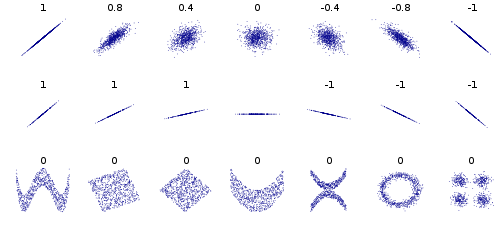
\includegraphics[width=0.8\linewidth]{images/Cor} 

}

\caption{Different forms of dependence and their ACF values}\label{fig:unnamed-chunk-4}
\end{figure}

It is worth noting that correlation does NOT imply causation. For
example, if \(\rho(t, t+h) \neq 0\), it does not imply that
\(X_t \to X_{t+h}\) is causal. Actually, real causation doesn't exist in
statistics but there exists approximated metric to measure this concept
such as Granger causality (see \citet{granger1969investigating}). This
idea is clearly illustrated in the image below:

\begin{figure}

{\centering 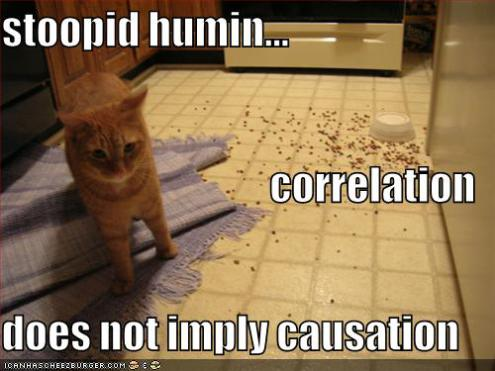
\includegraphics[width=0.5\linewidth]{images/corr_cat} 

}

\caption{Correlation does NOT imply causation.}\label{fig:unnamed-chunk-5}
\end{figure}

\hypertarget{stationarity}{%
\section{Stationarity}\label{stationarity}}

In this section we are going to introduce the concept of stationarity,
one of the most important characteristics of time series data. First let
us consider an example of \textbf{non-stationary processes}.

\BeginKnitrBlock{example}[Non-Stationary Process]
\protect\hypertarget{exm:exampleNonStationary}{}{\label{exm:exampleNonStationary}
\iffalse (Non-Stationary Process) \fi{} }\begin{equation*}
X_t  \sim \mathcal{N} \left(0, Y_t^2\right) \;\; \text{where $Y_t$ is unobserved and such that} \;\; Y_t  \overset{iid}{\sim} \mathcal{N} \left(0, 1\right).
\end{equation*}

In this case, it is clear that the estimation of \(\text{Var}(X_t)\) is
difficult since only \(X_t\) is useful for the estimation. So in fact,
\(X_t^2\) is our best guess for \(\text{Var}(X_t)\).
\EndKnitrBlock{example}

On the other hand, let us consider an example of \textbf{stationary
processes} where averaging becomes meaningful for such process.

\BeginKnitrBlock{example}[Stationary Process]
\protect\hypertarget{exm:exampleStationary}{}{\label{exm:exampleStationary}
\iffalse (Stationary Process) \fi{} }\begin{equation*}
X_t = \theta W_{t-1} + W_t \;\;\; \text{where} \;\;\;  W_t  \stackrel{iid}{\sim} \mathcal{N} \left(0, 1\right).
\end{equation*}

In this case, we can guess that a natural estimator of
\(\text{Var}(X_t)\) can be
\(\hat{\sigma}^2 = \frac{1}{T} \sum_{i = 1}^T X_i^2\). That is, now
averages are meaningful for such process.
\EndKnitrBlock{example}

We formalize the above idea by introducing the concept of stationarity.
There exist two forms of stationarity, which are defined below:

\BeginKnitrBlock{definition}[Strong Stationarity]
\protect\hypertarget{def:StrongStationarity}{}{\label{def:StrongStationarity}
\iffalse (Strong Stationarity) \fi{} }The time series \(X_{t}\) is
strongly stationary if the joint probability distribution is invariant
under a shift in time, i.e. \begin{equation*}
\mathbb{P}(X_{t}\leq x_{0},\ldots,X_{t+k}\leq x_{k}) = \mathbb{P}(X_{t+h}\leq x_{0} ,\ldots,X_{t+h+k}\leq x_{k})
\end{equation*} for any time shift \(h\) and any
\(x_{0}, x_{1},x_{2},\cdots,x_{k}\) belong to the domain of
\(X_t,\cdots,X_{t+k}\) and \(X_{t+h},\cdots,X_{t+h+k}\).
\EndKnitrBlock{definition}

\BeginKnitrBlock{definition}[Weak Stationarity]
\protect\hypertarget{def:WeakStationarity}{}{\label{def:WeakStationarity}
\iffalse (Weak Stationarity) \fi{} }The time series
\((X_{t})_{t \in \mathbb{N}}\) is weakly stationary if the mean and
autocovariance are finite and invariant under a shift in time, i.e.
\begin{equation*}
\begin{aligned}
\mathbb{E}\left[X_t\right] &= \mu < \infty,\\
\mathbb{E}\left[X_t^2\right]  &= \mu_2 < \infty,\\
\text{Cov}(X_{t},X_{t+h})&= \text{Cov}(X_{t + k},X_{t+h + k}) = \gamma( h ).
\end{aligned}
\end{equation*} for any time shift \(h\). For convenience, we use the
abbreviation ``stationary'' to indicate ``weakly stationary'' by
default.
\EndKnitrBlock{definition}

The stationarity of \(X_{t}\) is important because it provides a
framework in which averaging makes sense. The concept of averaging is
essentially meaningless unless properties like mean and covariance are
either fixed or evolve in a known manner.

\BeginKnitrBlock{exercise}[Implication on the ACV and ACF]
\protect\hypertarget{exr:StatImpAcvAcf}{}{\label{exr:StatImpAcvAcf}
\iffalse (Implication on the ACV and ACF) \fi{} }If a process is weakly
stationary or strongly stationary and \(\text{Cov}(X_{t},X_{t+h})\)
exists for all \(h \in \mathbb{Z}\), then we have both ACV and ACF only
depend on the lag between observations, i.e. \begin{equation*}
\begin{aligned}
\gamma(t, t+h) &= \text{Cov}(X_{t},X_{t+h})= \text{Cov}(X_{t + k},X_{t+h + k}) = \gamma(t+k, t+h+k) = \gamma(h),\\
\rho(t, t+h) &= \text{Corr}(X_{t},X_{t+h})= \text{Corr}(X_{t + k},X_{t+h + k}) = \rho(t+k, t+h+k) = \rho(h).
\end{aligned}
\end{equation*}
\EndKnitrBlock{exercise}

\BeginKnitrBlock{exercise}[Relation between Strong and Weak Stationarity]
\protect\hypertarget{exr:RelationStationary}{}{\label{exr:RelationStationary}
\iffalse (Relation between Strong and Weak Stationarity) \fi{} }

In general, neither type of stationarity implies the other one. However,

\begin{itemize}
\tightlist
\item
  If \(X_{t}\) is Normal (Gaussian) with
  \(\sigma^2 = \text{Var} (X_{t}) < \infty\), then weak stationarity
  implies strong stationarity.
\item
  If \(X_{t}\) is strongly stationary, \(\mathbb{E}(X_t) < \infty\) and
  \(\mathbb{E}(X_t^2) < \infty\), then \(X_{t}\) is weakly stationary.

  \EndKnitrBlock{exercise}
\end{itemize}

\BeginKnitrBlock{example}[Strong Stationarity does NOT imply Weak Stationarity]
\protect\hypertarget{exm:exampleRelationStat1}{}{\label{exm:exampleRelationStat1}
\iffalse (Strong Stationarity does NOT imply Weak Stationarity) \fi{}
}An iid Cauchy process is strongly but not weakly stationary as the mean
of the process does not exist.
\EndKnitrBlock{example}

\BeginKnitrBlock{example}[Weak Stationarity does NOT imply Strong Stationarity]
\protect\hypertarget{exm:exampleRelationStat2}{}{\label{exm:exampleRelationStat2}
\iffalse (Weak Stationarity does NOT imply Strong Stationarity) \fi{}
}Let \(X_t \overset{iid}{\sim} \exp(1)\) (i.e.~exponential distribution
with \(\lambda = 1\)) and \(Y_t \overset{iid}{\sim} \mathcal{N}(1,1)\).
Then, let \begin{equation*}
Z_t = \left\{
\begin{array}{cl}
X_t &\text{if } t \in \left\{2k | k \in \mathbb{N}\right\}\\
Y_t &\text{if }  t \in \left\{2k + 1 | k \in \mathbb{N}\right\},
\end{array}
\right.
\end{equation*} we have \(Z_t\) is weakly stationary but not strongly
stationary.
\EndKnitrBlock{example}

\BeginKnitrBlock{exercise}[Stationarity of Latent Time Series Processes]
\protect\hypertarget{exr:StatProcesses}{}{\label{exr:StatProcesses}
\iffalse (Stationarity of Latent Time Series Processes) \fi{} }

\begin{itemize}
\tightlist
\item
  (Weakly) Stationary: WN, QN, AR1
\item
  (Weakly) Non-Stationary: DR, RW

  \EndKnitrBlock{exercise}
\end{itemize}

\BeginKnitrBlock{proof}[AR1 is weakly stationary]
\iffalse{} {Proof (AR1 is weakly stationary). } \fi{}Consider an AR1
process defined as: \begin{equation*}
X_t = \phi X_{t-1} + Z_t, \;\;\; Z_t \overset{iid}{\sim} \mathcal{N}(0,\nu^2),
\end{equation*} where \(\mid \phi \mid < 1\) and \(\nu^2 < \infty\).
Then we have \[\begin{aligned}
{X_t}  &=   {\phi }{X_{t - 1}} + {Z_t} = \phi \left[ {\phi {X_{t - 2}} + {Z_{t - 1}}} \right] + {Z_t} =  {\phi ^2}{X_{t - 2}} + \phi {Z_{t - 1}} + {Z_t}  \\
& \; \vdots  \\
&=   {\phi ^k}{X_{t-k}} + \sum\limits_{j = 0}^{k - 1} {{\phi ^j}{Z_{t - j}}} .
\end{aligned} \] By taking the limit in \(k\) (which is perfectly valid
as we assume \(t \in \mathbb{Z}\)), we obtain \begin{equation*}
\begin{aligned}
X_t = \mathop {\lim }\limits_{k \to \infty} \; {X_t}  =  \sum\limits_{j = 0}^{\infty} {{\phi ^j}{Z_{t - j}}}.
\end{aligned}
\end{equation*} So we have \begin{equation*}
\begin{aligned}
\mathbb{E}\left[X_t\right] &=  \sum\limits_{j = 0}^{\infty} {{\phi ^j}{\mathbb{E} [Z_{t - j}]}} = 0, \\
\text{Var}\left(X_t\right) &= \text{Var}\left(\sum\limits_{j = 0}^{\infty} {{\phi ^j}{Z_{t - j}}}\right) = \sum\limits_{j = 0}^{\infty} {\phi^{2j}} \text{Var}\left(Z_{t-j}\right) = \nu^2 \sum\limits_{j = 0}^{\infty} {\phi^{2j}} = \frac{\nu^2}{1-\phi^2} < \infty.
\end{aligned}
\end{equation*} Moreover, assuming for notational simplicity that
\(h > 1\), we obtain \begin{equation*}
\begin{aligned}
\text{Cov}\left(X_t, X_{t+h}\right) &= \phi \text{Cov}\left(X_t, X_{t+h-1}\right) = \phi^2 \text{Cov}\left(X_t, X_{t+h-2}\right) = \ldots = \phi^h \text{Cov}(X_t, X_t).
\end{aligned}
\end{equation*} In general, when \(h \in \mathbb{Z}\) we obtain
\begin{equation*}
\begin{aligned}
\text{Cov}\left(X_t, X_{t+h}\right) & = \phi^{|h|} \text{Cov}(X_t, X_t) = \phi^{|h|} \frac{\nu^2}{1-\phi^2},
\end{aligned}
\end{equation*} which is a function of the lag \(h\) only. Therefore,
this AR1 process is weakly stationary.
\EndKnitrBlock{proof}

\hypertarget{linear-processes}{%
\section{Linear Processes}\label{linear-processes}}

In this section we introduce the concept of linear processes. As a
matter of fact, the stationary models considered so far can all be
represented as linear processes.

\BeginKnitrBlock{definition}[Linear Processes]
\protect\hypertarget{def:LinearProc}{}{\label{def:LinearProc}
\iffalse (Linear Processes) \fi{} }A stochastic process \((X_t)\) is
said to be a linear process if it can be expressed as a linear
combination of an iid Gaussian sequence (i.e.~white noise process),
i.e.:
\[{X_t} = \mu + \sum\limits_{j =  - \infty }^\infty  {{\psi _j}{W_{t - j}}} \]
where \(W_t \overset{iid}{\sim} \mathcal{N}(0, \sigma^2)\) and
\(\sum\limits_{j = - \infty }^\infty {\left| {{\psi _j}} \right|} < \infty\).
\EndKnitrBlock{definition}

Notice that the condition
\(\sum\limits_{j = - \infty }^\infty {\left| {{\psi _j}} \right|} < \infty\)
is required in the definition of linear processes in order to ensure
that the series has a limit and is related to the absolutely summable
covariance structure, which is defined below.

\BeginKnitrBlock{definition}[Absolutely Summable Covariance Structure]
\protect\hypertarget{def:AbsSumCov}{}{\label{def:AbsSumCov}
\iffalse (Absolutely Summable Covariance Structure) \fi{} }A process
\((X_t)\) is said to have an absolutely summable covariance structure if
\(\sum\limits_{h = - \infty }^\infty {\left| \gamma_X(h) \right|} < \infty\).
\EndKnitrBlock{definition}

\BeginKnitrBlock{exercise}[Properties of Linear Processes]
\protect\hypertarget{exr:propertiesLinearProc}{}{\label{exr:propertiesLinearProc}
\iffalse (Properties of Linear Processes) \fi{} }

\begin{enumerate}
\def\labelenumi{\arabic{enumi}.}
\item
  All linear processes are stationary since \[\begin{aligned}
  \mathbb{E}[X_t] &= \mu, \\
  \gamma(h) &= \sigma^2\sum\limits_{j =  - \infty }^\infty  {{\psi _j}{\psi _{j+h}}}.
  \end{aligned}\]
\item
  All linear processes have absolutely summable covariance structures.

  \EndKnitrBlock{exercise}
\end{enumerate}

\BeginKnitrBlock{proof}[ACV of Linear Processes]
\iffalse{} {Proof (ACV of Linear Processes). } \fi{}\begin{align*}
\gamma(h) &= \text{Cov}(X_t, X_{t+h}) = \text{Cov}(\mu+\sum_{j=-\infty}^{\infty} \psi_j W_{t-j}, \mu+\sum_{j=-\infty}^{\infty} \psi_j W_{t+h-j})\\
&= \text{Cov}(\sum_{j=-\infty}^{\infty} \psi_j W_{t-j}, \sum_{j=-\infty}^{\infty} \psi_j W_{t-(j-h)}) \\
&= \text{Cov}(\sum_{j=-\infty}^{\infty} \psi_j W_{t-j}, \sum_{j=-\infty}^{\infty} \psi_{j+h} W_{t-j}) \\
&= \sum_{j=-\infty}^{\infty} \psi_j \psi_{j+h} \text{Cov}(W_{t-j}, W_{t-j}) \\
&= \sigma^2\sum\limits_{j =  - \infty }^\infty  {{\psi _j}{\psi _{j+h}}}.
\end{align*}
\EndKnitrBlock{proof}

\BeginKnitrBlock{proof}[All linear processes have absolutely summable covariance structures]
\iffalse{} {Proof (All linear processes have absolutely summable
covariance structures.). } \fi{}\begin{align*}
\sum_{h=-\infty}^{\infty} \mid \gamma(h) \mid &= \sum_{h=-\infty}^{\infty} \sigma^2 \mid \sum_{j=-\infty}^{\infty} \psi_j \psi_{j+h} \mid \\
&\leq \sigma^2 \sum_{h=-\infty}^{\infty} \sum_{j=-\infty}^{\infty} \mid \psi_j \psi_{j+h} \mid \\
&= \sigma^2 \sum_{j=-\infty}^{\infty} \sum_{h=-\infty}^{\infty} \mid \psi_j \mid \cdot \mid \psi_{j+h} \mid \\
&= \sigma^2 \sum_{j=-\infty}^{\infty} \mid \psi_j \mid \sum_{h=-\infty}^{\infty} \mid \psi_{j+h} \mid \\
&= \sigma^2 \big( \sum_{j=-\infty}^{\infty} \mid \psi_j \mid \big)^2 < \infty
\end{align*} So with the assumption that
\(\sum_{j=-\infty}^{\infty} \mid \psi_j \mid < \infty\), we obtain that
all linear processes have absolutely summable covariance structures.
Notice that here we have shown that the condition
\(\sum\limits_{j = - \infty }^\infty {\left| {{\psi _j}} \right|} < \infty\)
is actually stronger than
\(\sum\limits_{h = - \infty }^\infty {\left| \gamma(h) \right|} < \infty\).
\EndKnitrBlock{proof}

\BeginKnitrBlock{example}[AR1 is a linear process]
\protect\hypertarget{exm:AR1isLP}{}{\label{exm:AR1isLP} \iffalse (AR1 is a
linear process) \fi{} }When we prove above that AR1 is weakly
stationary, we have shown that for an AR1 process
\(X_t = \phi X_{t-1} + Z_t, \;\;\; Z_t \overset{iid}{\sim} \mathcal{N}(0,\nu^2)\),
it can be represented as \begin{align*}
X_t = \sum\limits_{j = 0}^{\infty} {{\phi ^j}{Z_{t - j}}}.
\end{align*} Therefore, AR1 is a linear process.
\EndKnitrBlock{example}

\hypertarget{fundamental-representations-of-time-series}{%
\section{Fundamental Representations of Time
Series}\label{fundamental-representations-of-time-series}}

We conclude this chapter by summarizing the fundamental representations
of time series. If two processes have the same fundamental
representations, then these two processes are the same. There are two
most commonly used fundamental representations of time series, i.e.

\begin{itemize}
\tightlist
\item
  ACV and ACF;
\item
  the Power Spectral Density (PSD).
\end{itemize}

\BeginKnitrBlock{exercise}[ACV and ACF as fundamental representation]
\protect\hypertarget{exr:FundaRepreACVACF}{}{\label{exr:FundaRepreACVACF}
\iffalse (ACV and ACF as fundamental representation) \fi{} }If we
consider a zero mean normally distributed process, it is clear that its
joint distribution is fully characterized by the autocovariances
\(\mathbb{E}[X_t X_{t+h}]\) since the joint probability density only
depends on these covariances. Once we know the autocovariances we know
everything there is to know about the process and therefore: if two
processes have the same autocovariance function, then they are the same
process.
\EndKnitrBlock{exercise}

\BeginKnitrBlock{exercise}[PSD as fundamental representation]
\protect\hypertarget{exr:FundaReprePSD}{}{\label{exr:FundaReprePSD}
\iffalse (PSD as fundamental representation) \fi{} }The Power Spectral
Density (PSD) is defined as \begin{equation*}
    S_X(f) = \int_{- \infty}^{\infty} \gamma_{X}(h)\,e^{-ifh}dh,
\end{equation*} where \(f\) is a frequency. Hence, the PSD is a Fourier
transform of the autocovariance function which describes the variance of
a time series over frequencies (with respect to lags \(h\)).

Given that the definition of the PSD, as for the autocovariance
function, once we know the PSD we know everything there is to know about
the process and therefore: if two processes have the same PSD, then they
are the same process.
\EndKnitrBlock{exercise}

\hypertarget{a-review-of-the-properties-of-statistical-estimators}{%
\chapter{A Review of the Properties of Statistical
Estimators}\label{a-review-of-the-properties-of-statistical-estimators}}

TO DO

\hypertarget{allan-variance-calibration-techniques}{%
\chapter{Allan Variance Calibration
Techniques}\label{allan-variance-calibration-techniques}}

\begin{itemize}
\tightlist
\item
  The Allan Variance (AV) is a statistical technique originally
  developed in the mid-1960s to study the stability of precision
  oscillators \citep[see e.g.][]{allan1966statistics}.
\item
  It can provide information on the types and magnitude of various
  superimposed noise terms (i.e.~composite stochastic processes).
\item
  This method has been adapted to characterize the properties of a
  variety of devices including inertial sensors
  \citep[see][]{elsheimy08av}.
\item
  The AV is a measure of variability developed for long term memory
  processes and can in fact be interpreted as a Haar wavelet coefficient
  variance \citep[see][]{percival1994long}. We will discuss this
  connection further on.
\end{itemize}

\BeginKnitrBlock{definition}[Allan Variance]
\protect\hypertarget{def:defAV}{}{\label{def:defAV} \iffalse (Allan
Variance) \fi{} }We consider the AV at dyadic scales (\(\tau_j\))
starting from local averages of the process which can be denoted as

\begin{equation*} 
    \bar{X}_{t}^{(j)} \equiv \frac{1}{\tau_j} \sum_{i = 1}^{\tau_j} X_{t - \tau_j + i}\, ,
    \label{mean.noav}
\end{equation*}

where
\(\tau_j \equiv 2^j, \; j \in \left\{x \in \mathbb{N} \, : \; 1 \leq x < \log_2 (T) - 1 \right\}\)
therefore determines the number of consecutive observations considered
for the average. Then, the AV is defined as

\begin{equation*}
    \text{AV}_j \left(X_t \right) \equiv \frac{1}{2} \, \mathbb{E}\left[ \left(\bar{X}_{t}^{(j)} - \bar{X}_{t-\tau_j}^{(j)} \right)^2 \right].
\end{equation*}
\EndKnitrBlock{definition}

\BeginKnitrBlock{exercise}[Alternative scale definition]
\protect\hypertarget{exr:alterDefScale}{}{\label{exr:alterDefScale}
\iffalse (Alternative scale definition) \fi{} }The definition of the AV
is actually valid for \(\tau_j = \lfloor2^j\rfloor\) with
\(j \in \left\{x \in \mathbb{R} \, : \; 1 \leq x < \log_2 (T) - 1 \right\}\).
In some case, it could use to consider this alternative definition
\citep[see e.g.][]{elsheimy08av} but we shall restrict ourself here to
the case where
\(j \in \left\{x \in \mathbb{N} \, : \; 1 \leq x < \log_2 (T) - 1 \right\}\).
\EndKnitrBlock{exercise}

\BeginKnitrBlock{exercise}[Notation of the Allan Variance]
\protect\hypertarget{exr:notationAV}{}{\label{exr:notationAV}
\iffalse (Notation of the Allan Variance) \fi{} }For notational
simplicity, we may sometimes replace \(\text{AV}_j \left(X_t \right)\)
by simply \(\phi_j^2\) when the dependence of the AV to the process
\((X_t)\) is evident.
\EndKnitrBlock{exercise}

As highlighted earlier, the AV is, among others, a widely and commonly
used approach in engineering for sensor calibration as it is linked to
the properties of the process \((X_t)\) as shown in the following lemma
\citep[see e.g.][ for a proof]{percival2006wavelet}.

\BeginKnitrBlock{lemma}[AV connection to PSD]
\protect\hypertarget{lem:lemmavpsd}{}{\label{lem:lemmavpsd} \iffalse (AV
connection to PSD) \fi{} }For a stationary process \((X_t)\) with PSD
\(S_{X}(f)\) we have

\begin{equation*}
\phi_j^2 \equiv \text{AV}_j \left(X_t \right) = 4  \int_0^{\infty}  \frac{\sin^4(\pi f \tau_j)}{(\pi f \tau_j)^2} S_{X}(f) df. 
\label{eq:allanvariancePSD_LInk}
\end{equation*}
\EndKnitrBlock{lemma}

Therefore, this result establishes a direct connection between the AV
and PSD. A natural question is therefore whether the mapping PSD
\(\mapsto\) AV is one-to-one. \citet{greenhall1998spectral} (see Theorem
1) showed that this is actually not the case. This is illustrated in the
following section ????? (ADD REF).

\hypertarget{spectral-ambiguity-of-the-av}{%
\section{Spectral Ambiguity of the
AV}\label{spectral-ambiguity-of-the-av}}

Consider two (independent) stochastic processes \((X_t)\) and \((Y_t)\)
with respective PSD \(S_X(f)\) and \(S_Y(f)\). Suppose that
\(S_X(f) \neq S_Y(f)\), then the two processes will have the same AV if

\begin{equation*}
     \Delta \equiv \int_0^{\infty}  \frac{\sin^4(\pi f \tau_j)}{(\pi f \tau_j)^2} \Phi(f) df = 0,
\end{equation*}

where \(\Phi(f) \equiv S_{X}(f) - S_{Y}(f)\). To show that it is
possible that \(\Delta = 0\) when \(\Phi(f) \neq 0\), we will use the
following critical identity:

\begin{equation}
    \label{ident:av:indet}
    \sin^4(x) = \sin^2(x) - \frac{1}{4} \sin^2(2x).
\end{equation}

First, we note that \(\Delta\) may be expressed using
(\ref{ident:av:indet}) as follows: \begin{equation*}
    \begin{aligned}
        \Delta &=  \int_{0}^{\infty} \frac{\sin^4\left(\tau \pi f \right)}{\left(\tau \pi f \right)^2} \Phi(f) df \\
        &= \lim_{n \rightarrow -\infty} \int_{2^{n}}^{\infty} \frac{\sin^2\left(\tau \pi f \right) - \frac{1}{4} \sin^2\left(2 \tau \pi f \right) }{\left(\tau \pi f \right)^2} \Phi(f) df .
    \end{aligned}
\end{equation*}

Second, by the change of variable \(u = 2f\) in the second term we
obtain

\begin{equation*}
    \begin{aligned}
        \Delta = \lim_{n \rightarrow -\infty} & \Bigg[ \int_{2^{n}}^{\infty} \frac{\sin^2\left(\tau \pi f \right)}{\left(\tau \pi f \right)^2} \Phi(f) df - \frac{1}{2}\int_{2^{n+1}}^{\infty} \frac{\sin^2\left(\tau \pi u \right)}{\left(\tau \pi u \right)^2} \Phi(f) du \Bigg].
    \end{aligned}
\end{equation*}

Now suppose that \(\Phi(f) = 2 \Phi(2f)\). In this case, we have
\(\Phi(f) = 2 \Phi(u)\) and therefore we obtain \begin{equation*}
    \begin{aligned}
        \Delta &= \lim_{n \rightarrow -\infty} \int_{2^{n}}^{2^{n+1}} \frac{\sin^2\left(\tau \pi f \right)}{\left(\tau \pi f \right)^2} \Phi(f) df = 0.
    \end{aligned}
\end{equation*}

\BeginKnitrBlock{exercise}
\protect\hypertarget{exr:unnamed-chunk-6}{}{\label{exr:unnamed-chunk-6}
}This result demonstrates that the mapping from PSD to Allan variance is
not necessarily one-to-one. \citet{greenhall1998spectral} showed that in
the continuous case (i.e. \(\tau_j \in \mathbb{R}\)) \(\Delta = 0\) if
and only if \(\Phi(f) = 2 \Phi(2f)\). However, the ``only if'' part of
this results (while conjectured) is unknown in the discrete case.
\EndKnitrBlock{exercise}

\hypertarget{properties-of-the-allan-variance}{%
\section{Properties of the Allan
Variance}\label{properties-of-the-allan-variance}}

One reason of explaining the widespread use of the Allan variance for
sensor calibration is due to the following additivity property, which is
particularly convenient to identify composite stochastic processes (see
Definition REF MISSING!).

\BeginKnitrBlock{corollary}[Additivity of the AV]
\protect\hypertarget{cor:coroaddav}{}{\label{cor:coroaddav}
\iffalse (Additivity of the AV) \fi{} }Consider two (independent)
stochastic processes \((X_t)\) and \((Y_t)\) with respective PSD
\(S_X(f)\) and \(S_Y(f)\). Suppose that we observe the process
\(Z_t = X_t + Y_t\). Then, we have

\begin{equation*}
    \text{AV}_j \left(Z_t \right) = \text{AV}_j \left(X_t \right) + \text{AV}_j \left(Y_t \right).
\end{equation*}
\EndKnitrBlock{corollary}

\BeginKnitrBlock{proof}
\iffalse{} {Proof. } \fi{}The proof of this result is direct from Lemma
REF MISSING HERE. Indeed, since \(S_Z(f) = S_X(f) + S_Y(f)\), we have

\begin{equation*}
    \begin{aligned}
    \text{AV}_j \left(Z_t \right) &= 4  \int_0^{\infty}  \frac{\sin^4(\pi f \tau_j)}{(\pi f \tau_j)^2} S_{Z}(f) df\\
    &= 4  \int_0^{\infty}  \frac{\sin^4(\pi f \tau_j)}{(\pi f \tau_j)^2} S_{X}(f) df + 4  \int_0^{\infty}  \frac{\sin^4(\pi f \tau_j)}{(\pi f \tau_j)^2} S_{Y}(f) df\\
    &= \text{AV}_j \left(X_t \right) + \text{AV}_j \left(Y_t \right).
    \end{aligned}
\end{equation*}
\EndKnitrBlock{proof}

While Lemma \ref{lem:lemmavpsd} is an important results which is very
convenient to determine the theoretical AV of a certain stochastic
process. However, the applicability of this results is often limited
since the integral defined in (REF MISSING HERE) can be intractable. An
alternative to Lemma \ref{lem:lemmavpsd} has been proposed by
\citet{zhang2008allan} and is far advantageous from a computational
standpoint.

\BeginKnitrBlock{lemma}[AV connection to ACF]
\protect\hypertarget{lem:lemmaavtoacf}{}{\label{lem:lemmaavtoacf}
\iffalse (AV connection to ACF) \fi{} }For a stationary process
\((X_t)\) with variance \(\sigma^2_X\) and ACF \(\rho(h)\) we have
\begin{equation*}
\label{stat.av}
    \text{AV}_j \left(X_t \right)  = \frac{\sigma_X^2}{\tau_j^2} \bigg(\tau_j\left[1-\rho(\tau_j)\right] 
   + \sum_{i=1}^{\tau_j-1} i \left[2 \rho(\tau_j-i) - \rho(i) - \rho(2\tau_j-i)\right]\bigg).
\end{equation*}
\EndKnitrBlock{lemma}

The proof of this result is instructive and is presented in
\citet{xu2017study}.

\BeginKnitrBlock{exercise}
\protect\hypertarget{exr:unnamed-chunk-8}{}{\label{exr:unnamed-chunk-8}
}Using Lemma \ref{lem:lemmaavtoacf}, the exact form of the AV for
different stationary processes, such as the general class of ARMA
models, can easily be derived. Moreover, \citet{zhang2008allan} provided
the theoretical AV for non-stationary processes such as the random walk
and ARFIMA models for which the AV, as mentioned earlier, represents a
better measure of uncertainty compared to other methods.
\EndKnitrBlock{exercise}

\BeginKnitrBlock{exercise}
\protect\hypertarget{exr:unnamed-chunk-9}{}{\label{exr:unnamed-chunk-9}
}Lemma \ref{lem:lemmaavtoacf} was extended to non-stationary processes
in \citet{xu2017study}.
\EndKnitrBlock{exercise}

\BeginKnitrBlock{example}[Theoretical AV of an MA(1) process]
\protect\hypertarget{exm:avma1}{}{\label{exm:avma1} \iffalse (Theoretical AV
of an MA(1) process) \fi{} }From the autocovariance we obtain

\begin{equation*}
        \rho(h) = \text{corr}\left(X_t, X_{t-h} \right) =\left\{
  \begin{array}{cl}
    1 &\text{if } h = 0\\
    \frac{\theta}{1 + \theta^2} &\text{if } |h| = 1\\
    0 &\text{if } |h| > 1.\\
  \end{array}
\right.
\end{equation*}

We can now apply the formula given in Lemma \ref{lem:lemmaavtoacf},
which leads to

\begin{equation*}
    \begin{aligned}
        \text{AV}_j \left(X_t \right)  &= \frac{\left(1 + \theta^2 \right) \sigma^2}{\tau_j^2} \bigg(\tau_j
   + \sum_{i=1}^{\tau_j-1} i \left[2 \rho(\tau_j-i) - \rho(i) - \rho(2\tau_j-i)\right]\bigg)\\
   &=\frac{\left(1 + \theta^2 \right) \sigma^2}{\tau_j^2} \bigg(\tau_j
   + 2 \sum_{i=1}^{\tau_j-1} i \rho(\tau_j-i) -\sum_{i=1}^{\tau_j-1} i \rho(i) - \sum_{i=1}^{\tau_j-1} i \rho(2\tau_j-i)\bigg)\\
   &=\frac{\left(1 + \theta^2 \right) \sigma^2}{\tau_j^2} \left(\tau_j
   + 2  (\tau_j - 1) \rho(1) -  \rho(1) \right)\\
   &=\frac{\left(1 + \theta^2 \right) \sigma^2}{\tau_j^2} \bigg(\tau_j
   +  (2\tau_j - 3) \frac{\theta}{1 + \theta^2} \bigg).
   \end{aligned}
\end{equation*}

\(\LARGE{\bullet}\)
\EndKnitrBlock{example}

\hypertarget{estimation}{%
\section{Estimation}\label{estimation}}

Several estimators of the AV have been introduced in the literature. The
most commonly is (probably) the Maximum-Overlapping AV (MOAV) estimator
proposed by \citet{percival1994long}, which is defined as follows:

\BeginKnitrBlock{definition}[Maximum-Overlapping AV Estimator]
\protect\hypertarget{def:defmoav}{}{\label{def:defmoav}
\iffalse (Maximum-Overlapping AV Estimator) \fi{} }The MOAV is defined
as: \begin{eqnarray}
\label{eq:MOAVNS_est}
        \hat{\phi}_j^2 \equiv \widehat{\text{AV}}_j \left(X_t \right) = \frac{1}{2 \left(T - 2\tau_j + 1\right)} \sum_{k = 2 \tau_j}^{T} \left(\bar{X}_{k}^{(j)} - \bar{X}_{k-\tau_j}^{(j)} \right)^2.
\end{eqnarray}
\EndKnitrBlock{definition}

We will now study the properties of this estimator through the following
lemmas.

\hypertarget{consistency}{%
\subsection{Consistency}\label{consistency}}

\BeginKnitrBlock{lemma}[Consistency]
\protect\hypertarget{lem:lemmconsistencyAV}{}{\label{lem:lemmconsistencyAV}
\iffalse (Consistency) \fi{} }Let \((X_t)\) be such that:

\begin{itemize}
\tightlist
\item
  \((X_t - X_{t-1})\) is a (strongly) stationary process,
\item
  \((X_t - X_{t-1})^2\) has absolutely summable covariance structure,
\item
  \(\mathbb{E}\left[(X_t - X_{t-1})^4\right] < \infty\),
\end{itemize}

Then, we have
\[\widehat{\text{AV}}_j \left(X_t \right) \overset{ \mathcal{P} }{\longrightarrow} \text{AV}_j \left(X_t \right).\]
\EndKnitrBlock{lemma}

\BeginKnitrBlock{proof}
\iffalse{} {Proof. } \fi{}TO BE ADDED
\EndKnitrBlock{proof}

\BeginKnitrBlock{exercise}[Connection to Wavelet Variance]
\protect\hypertarget{exr:unnamed-chunk-11}{}{\label{exr:unnamed-chunk-11}
\iffalse (Connection to Wavelet Variance) \fi{} }This result is closely
related by the results of \citet{percival1995estimation} on the wavelet
variance. We shall explore the connection between the AV and wavelet
variance in the next section.
\EndKnitrBlock{exercise}

\hypertarget{asymptotic-normality}{%
\subsection{Asymptotic Normality}\label{asymptotic-normality}}

Compare to consistency, the asymptotic normality requires stronger
conditions given in the following lemma.

\BeginKnitrBlock{lemma}[Asymptotic normality]
\protect\hypertarget{lem:lemmaasyav}{}{\label{lem:lemmaasyav}
\iffalse (Asymptotic normality) \fi{} }Let \((X_t)\) be such that:

\begin{itemize}
\tightlist
\item
  \((X_t - X_{t-1})\) is a (strongly) stationary process.
\item
  \((X_t - X_{t-1})\) is strong mixing process with mixing coefficient
  \(\alpha(n)\) such that
  \(\sum_{n=1}^{\infty} \alpha(n)^{\frac{\delta}{2+\delta}} < \infty\)
  for some \(\delta > 0\).
\item
  \(\mathbb{E}\left[\left(X_t - X_{t-1}\right)^{4+\delta}\right] < \infty\)
  for some \(\delta > 0\).
\end{itemize}

Then, under these conditions we have that
\[\sqrt{T}\left(\widehat{\text{AV}}_j \left(X_t \right) - \text{AV}_j \left(X_t \right) \right) \overset{ \mathcal{D} }{\longrightarrow}
\mathcal{N}(0, \sigma^2_T/T),\] where
\(\sigma^2_T \equiv \sum_{h = -\infty}^{\infty}\text{cov}\left( \left(\bar{X}_{t}^{(j)} - \bar{X}_{t-\tau_j}^{(j)} \right)^2, \left(\bar{X}_{t+h}^{(j)} - \bar{X}_{t+h-\tau_j}^{(j)} \right)^2 \right)\).
\EndKnitrBlock{lemma}

\BeginKnitrBlock{proof}
\iffalse{} {Proof. } \fi{}TO BE ADDED
\EndKnitrBlock{proof}

\hypertarget{confidence-interval-of-the-moav-estimator}{%
\subsection{Confidence Interval of the MOAV
Estimator}\label{confidence-interval-of-the-moav-estimator}}

Based on the asymptotic normality results (Lemma \ref{lemma:asy:av}), we
can construct the \(1-\alpha\) confidence intervals for
\(\widehat{\text{AV}}_j \left(X_t \right)\) as \% \begin{equation*}
    \text{CI}\left(\text{AV}_j \left(X_t \right)\right) = \left[ \widehat{\text{AV}}_j \left(X_t \right) \pm z_{1 - \frac{\alpha}{2}} \frac{\sigma_{T}}{T} \right],
\end{equation*} \% where
\(z_{1 - \frac{\alpha}{2}} \equiv \boldsymbol{\Phi}^{-1}\left( 1- \frac{\alpha}{2} \right)\)
is the \((1- \frac{\alpha}{2})\) quantile of a standard normal
distribution.\textbackslash{} However, the so called ``Long-Run
Variance'' \(\sigma^2_{T}\) is usually unknown. Many methods have been
proposed to consistently estimate it under mild conditions \citep[see
e.g.][]{newey1986simple}.

\BeginKnitrBlock{exercise}
\protect\hypertarget{exr:unnamed-chunk-13}{}{\label{exr:unnamed-chunk-13}
}Gaussian-based confidence intervals are often problematic with the AV
as the lower limit of CI can very well be negative. Next, we will
discuss an alternative method to construct the CI for such statistic.
\EndKnitrBlock{exercise}

\hypertarget{allan-variance-based-estimation}{%
\section{Allan variance based
estimation}\label{allan-variance-based-estimation}}

\hypertarget{allan-variance-log-log-representation}{%
\subsection{Allan Variance log-log
Representation}\label{allan-variance-log-log-representation}}

As illustrated in Lemmas \ref{lem:lemmavpsd} and \ref{lem:lemmaavtoacf}
the AV depends on the properties of the stochastic process \((X_t)\). We
will see that ``log-log'' representation of the AV is often useful for
the identify various processes that may compose \((X_t)\).

For example, let's suppose that \(X_t\) is a white noise process. We
showed in REF MISSING HERE that the theoretical AV of such process is
given

\begin{equation*}
      \phi_j^2 \equiv \text{AV}_j(X_t) = \frac{\sigma^2}{\tau_j}.
\end{equation*}

Therefore, we have that the Allan Deviation or AD (i.e.
\(\sqrt{\text{AV}_j(X_t)}\) or \(\phi_j\)) is such that

\begin{equation}
       \log\left( \phi_j \right) = \log \left(\sqrt{\frac{\sigma^2}{\tau_j}}\right) = \log \left(\sigma\right) - \frac{1}{2} \log (\tau_j).
       \label{eq:av:wn}
\end{equation}

Thus, the log of the AD is linear in \(\tau_j\) with a slope of \(-1/2\)
and with intercept \(\log (\sigma)\). Let us start by considering a
simple simulated example.

\hypertarget{allan-deviation-of-a-wn-process}{%
\subsection{Allan Deviation of a WN
process}\label{allan-deviation-of-a-wn-process}}

Simulation based on a white noise process with \(\sigma^2 = 10^2\) and
\(T = 10^5\).

\begin{Shaded}
\begin{Highlighting}[]
\CommentTok{# Load packages}
\KeywordTok{library}\NormalTok{(av)      }\CommentTok{# Package for Allan Variance functions}
\KeywordTok{library}\NormalTok{(simts)   }\CommentTok{# Package for time series simulations}

\CommentTok{# Simulate white noise}
\NormalTok{Xt =}\StringTok{ }\KeywordTok{gen_gts}\NormalTok{(}\KeywordTok{WN}\NormalTok{(}\DataTypeTok{sigma2 =} \DecValTok{1}\NormalTok{), }\DataTypeTok{n =} \DecValTok{10}\OperatorTok{^}\DecValTok{5}\NormalTok{)}

\CommentTok{# Compute allan variance}
\NormalTok{av =}\StringTok{ }\KeywordTok{avar}\NormalTok{(Xt)}

\CommentTok{# Allan Variance log-log Representation}
\KeywordTok{plot}\NormalTok{(av)}
\end{Highlighting}
\end{Shaded}

\begin{figure}

{\centering 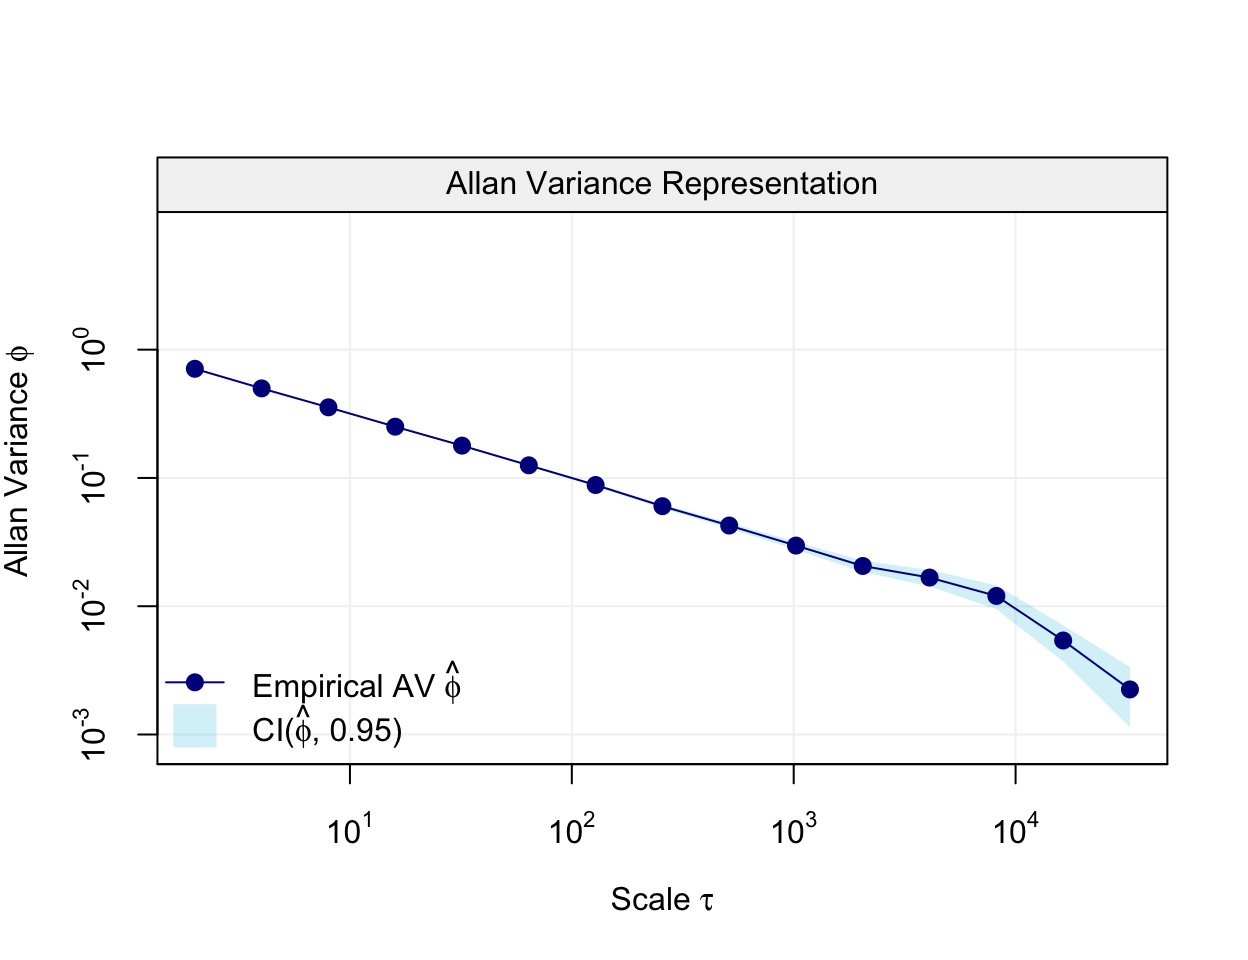
\includegraphics{scis_files/figure-latex/exampleAVwhitenoise-1} 

}

\caption{ADD A NICE CAPTION}\label{fig:exampleAVwhitenoise}
\end{figure}

\hypertarget{the-generalized-method-of-wavelet-moments}{%
\chapter{The Generalized Method of Wavelet
Moments}\label{the-generalized-method-of-wavelet-moments}}

\hypertarget{extensions}{%
\chapter{Extensions}\label{extensions}}

\bibliography{biblio.bib,book.bib,packages.bib}


\end{document}
